\end{multicols*}

\mysection{Wizardry}{arcana-wizardry}

\flavor{\myital{Klaatu barada nikto!} \\~ \Tilde "The Day the Earth Stood Still" / "Army of Darkness"}

    The Arcana of Wizardry allows you to perform \mylink{the Secrets}{arcana-wizardry-secrets} by using your \mylink{Blood Die}{cruces-blood-dice}. You can't spend your Blood Dice if there is too much iron nearby (see the section on the \mylink{Crux of Blood}{cruces-blood}). You must declare how many Blood Dice you are rolling before you invoke a Secret. If a Blood Die comes up a Failure (a 1 or a 2), it is immediately \mylink{Spent}{dice-spent}. How many Blood Die you roll is up to you - the more dice you roll, the more powerful the effect, but the higher the chance of catastrophe if you roll any triples, quadruples, or more.

Speaking a Secret inscribed in your cranium is a \mylink{Combat Action}{combat-combat-actions} that may take up to two Maneuver Actions to "prepare", depending on where the Secret is inscribed:

    \mybullet {
        \item If the Secret is inscribed on the inside of your skull (see below), it requires no Maneuvers to prepare;
        \item If the Secret is inscribed on a \mylink{Fetish}{fetishes}, it requires \mybold{1 Maneuver Action} to prepare; 
        \item If the Secret is inscribed in a \mylink{Grimoire}{grimoires}, it requires \mybold{2 Maneuver Actions} to find the right page (not including the time it takes to get it out of your bag) and speak the Secret. 
    }

    See the \mylink{Inscription}{research-inscription} section under \mylink{Research}{research} for more info about Fetishes and Grimoires.

\vspace{20mm}

\begin{multicols*}{2}

\mysubsection{The Sorcerer's Skull}{arcana-wizardry-skull}

Secrets inscribed in your skull can be spoken at any time - you simply "know" them, as you know your own name.

If you separate the skull from the Sorcerer and carefully scrape away the brains, you may use it as an extremely potent \mybold{Fetish} - one that doesn't have a \UD attached to it (meaning it doesn't lose potency with repeated use!). You cannot inscribe Secrets from a skull into a Grimoire or Fetish without removing the brain first.


\cbreak


\myimage{arcana/MushroomSkull}



\newpage

\end{multicols*}
\mysubsection{Components}{arcana-wizardry-components}

\flavor{I collect molds, spores, and fungus.  \\~ \Tilde Egon Spengler, "Ghostbusters"}

Eye of newt, toe of frog, etc. By collecting various ... uh, parts ... you might come across, you can augment your Secrets and make them easier to perform. Secrets require blood to perform "correctly", so these Components must come from a (once) living thing - often a Monster.

\mybold{If you invoke a Secret with a Component, you only Spend a Blood die if you roll a 1 (instead of a 1 or 2)}.  Components are Insignificant items. When the Component is Spent, it's consumed in a puff of smoke / blue flame / swarm of gnats etc.

Components can only be harvested from fresh corpses during a \mylink{Breather}{combat-resting-breather}. It has to be something you can reasonably carry (Arbiter's choice) - basilisk tongue, OK.  Green slime, not OK. 

Make an \RSTRY{\INT}. If you Fail, nothing happens. If you succeed, you gain one \UDD{d4} of a Component.

What the component might be is up to you. You could declare that "kobold's eyes" are the Component for the \mylink{Secret: Sleep}{secrets-sleep}, and if you succeed in your \RS try, then kobold's eyes are always a component for Sleep (note it on your Adventurer sheet). This is only true for \mybold{you} and not anyone else (someone else's version of Sleep needs boggart boogers or whatever). Only one Component can augment a Secret - if you decide that kobold's eyes are the Component for Sleep, then \myital{only} kobold's eyes can be used with Sleep.

When harvesting, Monsters will only provide one component. You can't say kobold's eyes help Secret: Magic Missile and kobold's tongues help cast Secret: Battering Beam. You can also only harvest once per distinct Monster - so if you kill 9 kobolds and 14 trolls then you only get two tries - once for kobolds, and once for trolls.  No matter how many Monsters there are, you can only harvest one distinct \UDD{d4} of material from your each of your "donors".


\begin{multicols*}{2}

\crunch{Wizard Fight!}{arcana-wizardry-wizard-fight}

Some Secrets can be countered by other Secrets - for example, \mylink{Balthazar's Breathtaking Blast}{secrets-balthazars-breathtaking-blast} can be countered by \mylink{Mighty Lungs}{secrets-mighty-lungs}, and \mylink{Invisibility}{secrets-invisibility} can be dispelled by the wisps summoned in the \mylink{Fool's Fire}{secrets-fools-fire}.


If you attempt to counter a Secret and the Philosopher who cast it is not present (that is, not somewhere Close, Nearby, Far-Away, or Distant) you automatically succeed.  Otherwise, you enter into a duel with the other Philosopher.

Each Philosopher must \RBTRY{\INT}{\INT}, adding the number of \DICE invested in the Secret as a positive modifier.

\formula{Wizard Fight!}{
  \RB : \INT ~ \PLUS ~ \DICE
}

The winner's Secret stays, the loser's Secret goes.  Put another way:

\callout {\footnotesize{
\mybullet{
  \item If you are countering a Secret and you win, the Secret you're attempting to counter is dispelled and your Secret takes effect
  \item If you are countering a Secret and you lose, the Secret you're attempting to counter remains, and your Secret fizzles with no effect.
}}}

If you attempt to counter a Secret and you roll a \mylink{Calamity}{table-calamities} or \mylink{Ruin}{table-ruin}, the counterspell doesn't work.


\newpage

\end{multicols}
\mysubsection{The Secrets}{arcana-wizardry-secrets}

In order to manifest a Secret, you must declare and roll one or more \mylink{Blood Dice}{cruces-blood-dice}. How many dice you decide to roll is completely up to you; the more dice you roll, the more powerful the Secret - but the greater the chance that you \mylink{Spend}{dice-spent} multiple dice, or roll a \mylink{Mishap}{table-mishap}, \mylink{Calamity}{table-calamities}, or \mylink{Ruin}{table-ruin}.  See the section on \mylink{the Crux of Blood}{cruces-blood} for more info on the Blood Die.

You must declare the number of Blood you are investing a Secret \myital{before} you roll; and you can't spend your Blood Dice if there is too much iron nearby. In Combat, speaking a Secret is a \mylink{Combat Action}{combat-combat-actions}.

\myhighlight{\faAnkh Alignment}{arcana-wizardry-secrets-alignment}

The Secrets are divided into a pentagram, each point aligned with a particular aspect of the Dream:

\callout{\footnotesize{

\mybullet {
  \item \mybold{Secrets of Biomancy:} Secrets that affect or utilize biological components;
  \item \mybold{Secrets of the Elements:} Secrets that utilize the four basic elements (air, fire, earth, water) as well as other ”elemental” forces (acid, lightning, etc.);
  \item \mybold{Secrets of Entropy:} Secrets that tap into the chaos and disorder native to the Void to either create or remove Chaos from the Dream;
  \item \mybold{Secrets of Force:} Secrets that affect the material world in some way;
  \item \mybold{Secrets of the Mind:} Secrets that affect the minds/brains of intelligent creatures (including illusions and enchantments).
}}}


Certain Monsters have, and other abilities provide, immunity to Secrets from certain Alignments. In those cases, the immunity is to the Secret itself and not from a "side-effect" of that immunity.  For instance, \mylink{Mindless}{monster-trait-mindless} Monsters are immune to the effects of the Secrets of the Mind (so they couldn't be \mylink{Charmed}{secrets-charm}), but could be attacked by someone who was themselves Charmed.

\myhighlight{Duration}{arcana-wizardry-duration}

Some Secrets will have a \Duration associated with them; the \Duration depends on the number of \DICE invested in the invocation of the Secret:

  \myctrtable{Y Y} {
    \thead{\DICE}  & \thead{\Duration} \\
  } {
    1 & d4  \\
    2 & d6 \\
    3 & d8 \\
    4 & d10 \\
    5 & d12 \\
    6+ & d16 \\
  }


  \myhighlight{Splittable}{keyword-splittable}

  Spells that can be split can have their dice split up among up to \DICE targets.  Each target resolves the effect of the dice on them separately, but the \DICE are pooled when considering Mishaps, Calamities, and Ruin.

  \example {
    The Wizardry arcanum \mylink{Charm}{secrets-charm} is Splittable and allows you to "...ensorcel one or more Monsters whose \HD are less than or equal to \DICE". If you had a pool of 4 Blood Dice, you could use 3 dice on 1 Monster and 2 on another, 1 die on 4 Monsters, etc. with the additional requirement that the \DICE used on the Monster is equal to or greater than their \HD
  }


\myfpimage{arcana/Tome}

\WIZARDRY[
  Name=Acid Arrow,
  Link=secrets-acid-arrow,
  Alignment=Elements,
  Save=N,
  Duration=\DICE,
  Counter=None,
  Keywords=None,
  Target=Nearby or Far-Away Monster or Object
]

You throw an acidic arrow at a Monster or object. You must make a successful Attack action using your \INT (instead of \VIG or \DEX).  If you succeed: 

\mynumlist {
  \item If the target is wearing Armor, they must make a \UD check at the start of every Moment for the \Duration of the spell.  If they are using a shield, they may immediately \mylink{Sunder}{combat-deeds-sunder} it to nullify the spell; 
  \item If they are not wearing Armor, they take \DICE damage at the start of every Moment for the \Duration of the spell; 
  \item If the target is an object, it will melt a \DICE x 10cm cubic area of wood, metal, or stone.  
}

\WIZARDRY[
  Name=Arcadia's Bulwark,
  Link=secrets-arcadias-bulwark,
  Alignment=Mind,
  Save=N,
  Duration=Session,
  Counter=\mylink{Acid Arrow}{secrets-acid-arrow},
  Keywords=None,
  Target=Self
]


A spectral shield with a heraldic device of your choosing appears in the vicinity of your non-dominant arm.  The shield moves on its own to block Throw and Shoot weapons, and can absorb up to \SUMDICE + \DICE damage before it dissipates.  You can also \mylink{Sunder}{combat-deeds-sunder} this shield (like the Combat ability), which also causes it to dissipate. You can still cast spells while this shield is summoned.  An Acid Arrow fired into the shield will dispel it if a Wizard Fight! is lost.


\WIZARDRY[
  Name=Balthazar's Breathtaking Blast,
  Link=secrets-balthazars-breathtaking-blast,
  Alignment=Biomancy,
  Save=Y (negate),
  Duration=\DICE,
  Counter=\mylink{Mighty Lungs}{secrets-mighty-lungs} ,
  Keywords=None,
  Target=Nearby or Far-Away point
]

A marble-sized bead of shit lands at a Nearby or Far-Away point you select. You can cause the sphere to detonate at any time in \DICE Hours (including immediately). All creatures Close or Nearby the sphere's detonation must
Save or immediately become \mylink{Sickened}{effect-sickened}, and the area is filled with a thick green mist that lasts for \DICE Hours.  Any who enter the mist during this time must Save or become \mylink{Sickened}{effect-sickened}, though you smell it and see it before you're in it, so you won't stumble into it blindly.  Animals will avoid the area for the \Duration.  The Secret does not affect creatures with no sense of smell, mindless creatures, or creatures who habitually live in
filth (goblins, otyughs, etc.).  The mist can be dispelled by Mighty Lungs if a Wizard Fight! is lost.




\WIZARDRY[
  Name=Bastogne's Glamping Charm,
  Link=secrets-bastognes-glamping-charm,
  Alignment=Force,
  Save=N,
  Duration=Bivouac,
  Counter=\mylink{Morass}{secrets-morass} ,
  Keywords=None,
  Target=Close
]

\DICE-1 purple and gold tents appear in a circle around the campfire where you and your Band are taking a \mylink{Bivouac}{combat-resting-bivouac}. Each tent includes a bedroll, a sleeping platform, a cot, a candle, and a pair of warm slippers. 
A cookpot appears over the fire with a stew going, enough to provide Provisions for you and your Band, regardless of how many \DICE you spent. Any items removed from the tents instantly vanish. In the radius of the campfire the temperature is moderated very slightly, wind and rain are lessened, and vermin won't enter.  The tents are immune to casual attack, including from wandering Monsters (anyone sleeping outside the tents might not be so lucky). When the campfire goes out or the sun rises, the Glamping Charm disappears. The campsite can be utterly dispelled by Morass if a Wizard Fight! is lost.

\WIZARDRY[
  Name=Battering Beam,
  Link=secrets-battering-beam,
  Alignment=Force,
  Save=N,
  Duration=Concentration,
  Counter=\mylink{Battering Beam}{secrets-battering-beam},
  Keywords=Contested,
  Target=Close or Nearby Monster or Object
]


A beam of force erupts from your forehead and strikes something you can see, pushing it backwards. Every Moment, the creature or object is pushed 5m in the direction you are looking.  If it's an object, you can push up to \DICE
x100kg.  If it's a Monster, they can try to \RBTRY{\INT}{\VIG} with a -\DICE penalty to fight back. If you lose the \RB try, the Secret immediately ends - otherwise, the Secret lasts as long as you \mylink{Concentrate}{time-concentration}.  If the target cannot move backwards, it takes \DICE damage.  The Battering Beam can be dispelled by another Battering Beam if a Wizard Fight! is lost.




\WIZARDRY[
  Name=Cacophony,
  Link=secrets-cacophony,
  Alignment=Entropy,
  Save=Y (negate),
  Duration=\DICE,
  Counter=\mylink{Negasonic Bomb}{secrets-negasonic-bomb} ,
  Keywords=None,
  Target=Nearby or Far-Away point
]



You roll a small orb of Entropy to a point Nearby or Far-Away; the orb rolls silently and is hard to see.  At any time for the next \SUMDICE Hours, you can have the orb detonate with an incredibly loud clattering, wailing, and whistling. It is audible in clear air up to a \DICE km away. You can designate \DICE conditions under which the orb will detonate. For example, you could say "now"; "if anyone steps on it"; or "if water touches it".  The conditions must be obvious and must occur within 1m of the orb. Creatures Close to the detonation must Save or be \mylink{Concussed}{effect-concussed} for the \Duration. The Cacophony can be dispelled by a Negasonic Bomb if a Wizard Fight! is lost.





\WIZARDRY[
  Name=Charm,
  Link=secrets-charm,
  Alignment=Mind,
  Save=Y (negate),
  Duration=Session,
  Counter=\mylink{Charm}{secrets-charm} ,
  Keywords=Contested,
  Target=Close Monster(s)
]

\begin{wrapfigure}[15]{l}{0.35\textwidth}
    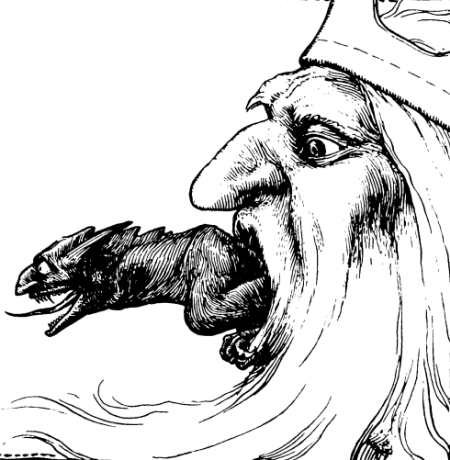
\includegraphics[scale=.35]{arcana/Tongue}
\end{wrapfigure}

Ensorcel one creature whose \HD is less than or equal to \DICE. You must touch the target's flesh (like with a handshake) when you speak the final word of this Secret. A successful \SAVE{Hexes} negates the effect; otherwise, they are \mylink{Charmed}{effect-charmed} and will regard you as a good friend and ignore the obvious enchantment you just cast on them.  The effect lasts for the entire Session unless you ask them to do something they might think was a little weird: attack an ally, let you through an area they're supposed to be guarding, etc. (this is up to the Arbiter's discretion).  This will prompt a
\RB your \INT vs. their \FOC with a -\DICE penalty. You can only have one creature Charmed at a time. The Charm can be broken and dispelled by another Charm if a Wizard Fight! is lost. 


\newpage

\WIZARDRY[
  Name=Color Spray,
  Link=secrets-color-spray,
  Alignment=Mind,
  Save=Y (negate),
  Duration=\DICE,
  Counter=None ,
  Keywords=Splittable,
  Target=Close or Nearby Monster(s)
]



You emit \DICE sprays of color from your fingertips that you can split among \DICE Monsters.  For each Monster, if the \SUMDICE of the \DICE targeting the Monster is twice as much (equal to or greater) as the Monster's \HD, it
is \mylink{Befuddled}{effect-befuddled} for the \Duration.  If \SUMDICE is three times the Monster's \HD, it is \mylink{Stunned}{effect-stunned} for a Moment, then \mylink{Befuddled}{effect-befuddled} as above. If \SUMDICE is five times the creature's \HD, it is \mylink{Stunned}{effect-stunned} for the Duration, then \mylink{Befuddled}{effect-befuddled} as above (reset the Duration die).  Save negates.





\WIZARDRY[
  Name=Commanding Presence,
  Link=secrets-commanding-presence,
  Alignment=Mind,
  Save=N,
  Duration=Combat or \SUMDICE real-world minutes,
  Counter=\mylink{Balthazar's Breathtaking Blast}{secrets-balthazars-breathtaking-blast} ,
  Keywords=None,
  Target=Self
]

You grow +\DICE meters in height, and your features and voice become terrible and commanding.  Creatures of less than \DICE \HD must test morale or flee in terror. For the duration of the Secret, you can use your \INT in place of any rolls where you would normally use \VIG.  If you enter the radius of Balthazar's Breathtaking Blast, or if the Secret is spoken Close to you, the Commanding Presence is dispelled if a Wizard Fight! is lost.




\WIZARDRY[
  Name=Ego Weapon,
  Link=secrets-ego-weapon,
  Alignment=Mind,
  Save=N,
  Duration=Session,
  Counter=\mylink{Greaseball}{secrets-greaseball} ,
  Keywords=None,
  Target=Self
]

You can summon a Bashing, Chopping, or Stabbing weapon of Force.  You can change the type of weapon by using 1 Action in Combat.  The weapon does \DICE damage and can hit creatures only affected by magic.  Only you can fight with the Ego Weapon.   You must make a successful Attack using your \INT (instead of \VIG or \DEX) to hit with the weapon.  A \mylink{Helping Hand}{secrets-helping-hand} can wield an Ego Weapon, but you can only have 1 Ego Weapon in existence at a time.  The weapon lasts for the entire Session.  It can be dispelled by a Greaseball if a Wizard Fight! is lost.

\WIZARDRY[
  Name=Enervate,
  Link=secrets-enervate,
  Alignment=Entropy,
  Save=Y (half),
  Duration=0,
  Counter=None ,
  Keywords=None,
  Target=Close or Nearby Magical Monster
]

On creatures that do not possess Blood or \mylink{Spell Dice}{monster-spell-dice}, this Secret has no effect.  Otherwise, the target of the Secret immediately takes \DICE damage for each unspent Blood/Spell Die they possess.

If 3 or more Blood Dice are spent on this Secret, the target must also immediately Save. Failure means they must immediately try \mybold{all} unspent Blood or Spell Dice as if they were manifesting them (any rolls of a 1 or a 2 loses the die; if you roll triples a Mishap occurs; etc.), though no magic will manifest.



\WIZARDRY[
  Name=Fireball,
  Link=secrets-fireball,
  Alignment=Elements,
  Save=Y (half),
  Duration=0,
  Counter=None ,
  Keywords=None,
  Target=Any point
]

You throw a ball of fire somewhere Close, Nearby, or Far Away.  Everyone Close to the detonation takes \SUMDICE+\DICE fire damage (Save for half), and highly flammable things are set aflame (curtains, dry trees, and oil but not people or buildings).




\WIZARDRY[
  Name=Fogbank,
  Link=secrets-fogbank,
  Alignment=Elements,
  Save=N,
  Duration=Concentration,
  Counter=\mylink{Mighty Lungs}{secrets-mighty-lungs} ,
  Keywords=None,
  Target=Close
]



You summon a bank of swirling and shifting fog that exists for as long as you Concentrate.  The fog can move with you, or you can take 2 Actions to mentally direct it somewhere Nearby.  The fog will blanket \SUMDICE creatures or a space \DICE+\DICE meters cubed.  Missiles that are thrown or shot into the fog strike a random target; nothing can be thrown or shot out of the fog.  The fog extinguishes small flames (torches, candles, etc). Monsters and Allies who attempt to fight while inside of the fog act as if they were \mylink{Befuddled}{effect-befuddled}.


\newpage


\WIZARDRY[
  Name=Fool's Fire,
  Link=secrets-fools-fire,
  Alignment=Entropy,
  Save=Y (negate),
  Duration=Concentration,
  Counter=\mylink{Enervate}{secrets-enervate} ,
  Keywords=Splittable,
  Target=Close or Nearby point
]

You project \DICE will-o'the-wisps into an area Close or Nearby.  The wisps can move one range (Close to Nearby, Nearby to Far Away, etc) in 1 Action.  You can split the wisps up any way you like but they can't be more than Far-Away from you.  The wisps do not shed heat, do not require air, and can't be doused by water.  They shed a steady yellow light the brightness of a torch.  At the top of the Moment, you can command up to \DICE wisps to \mylink{Befuddle}{effect-befuddled} up to \DICE Monsters that are Close to them.   Monsters get an initial Save and, if they succeed, the wisp targeting them is dispelled; otherwise, the Befuddlement lasts as long as you Concentrate. If any of the wisps are struck by an Enervate spell, they are all dispelled if a Wizard Fight! is lost.  When a wisp is dispelled, any Monsters \mylink{Befuddled}{effect-befuddled} by the wisp are released from the effect.

\WIZARDRY[
  Name=Greaseball,
  Link=secrets-greaseball,
  Alignment=Entropy,
  Save=N,
  Duration=\DICE,
  Counter=\mylink{Pritchard's Gusty Belch}{secrets-pritchards-gusty-belch} (acid) ,
  Keywords=None,
  Target=Close or Nearby Monster or Object
]

Toss a small ball of grease at a point on the ground Close or Nearby. If you would prefer to throw the ball at a person or object, make an Attack \RO using your \INT - if you miss, it dissipates.  If thrown at the ground, the surface becomes slick with a thick oil; anyone attempting to move through the area must \ROTRY{\DEX \PLUS \MD} with a -\DICE penalty, or immediately fall \mylink{Prone}{effect-prone}.  It requires a successful \RO as above to get up again.  

If you throw the Greaseball at a Monster, the effect is as above -  plus they can't hold anything without dropping it.  If you throw it at an object, the object becomes impossible to carry or hold until the grease is removed with an \mylink{Acid}{malignants-acids} (any strength), or is burned off. Pritchard's Gusty Belch (acid variety) will also dispel the grease if a Wizard Fight! is lost.  The grease is highly flammable. 

\newpage

\WIZARDRY[
  Name=Grimm's Electric Fingers,
  Link=secrets-grimms-electric-fingers,
  Alignment=Elements,
  Save=Y (half),
  Duration=0,
  Counter=None ,
  Keywords=None,
  Target=Close or Nearby Monster or Object
]

Forks of lightning erupt from your outstretched hands, striking a Close or Nearby target for \SUMDICE damage (Save for half). You can cause the
lightning to "jump" up to \DICE-1 times to another creature or object Close by, provided they are conductive (iron armor, metal ladders, etc).  Magic
swords aren't conductive.  You can "ping-pong" between two objects if you desire. Creatures struck by any bolt after the first take \DICE damage
(no Save). Objects struck by subordinate bolts will become momentarily electrified, and deal a shock that could cause someone to lose their grip unless they \RS using either their \VIG or \FOC.



\WIZARDRY[
  Name=Hammerspace Mule,
  Link=secrets-hammerspace-mule,
  Alignment=Force,
  Save=N,
  Duration=Session,
  Counter=\mylink{Illusion}{secrets-illusion} ,
  Keywords=Hammerspace,
  Target=Close
]

You create a spectral mule out of pure Force. The mule carries two \mylink{Hammerspace}{meta-hammerspace} saddlebags that can each hold \SUMDICE Burden whose combined weight doesn't exceed \DICE x 200kg (a reminder that a person is 25 Burden, and small creatures are 15).  The mule walks at a brisk trot.  It will stop and turn at your verbal command, but you cannot make it reverse or slow down. You can only give it the commands "go", "stop", "left", and "right". If the mule takes any damage, it immediately disappears and drops all the items on the ground.  The mule will obey your last command until the spell's duration expires.  Hammerspace Mules think that Illusions are real; if the Illusion would damage them in some way (a pit they would fall into, a spear they would run into, etc) the Mule is dispelled (dropping its items on the ground) if a Wizard Fight! is lost.


\WIZARDRY[
  Name=Helping Hand,
  Link=secrets-helping-hand,
  Alignment=Biomancy,
  Save=N,
  Duration=Concentration,
  Counter=\mylink{Web}{secrets-web} ,
  Keywords=None,
  Target=Self
]



You can detach either hand from its wrist.  The hand floats at chest height and can hold anything you could normally hold.  The hand can't use any weapons except for an \mylink{Ego Weapon}{secrets-ego-weapon}.  It can grab shirts, press buttons, and shove people (but not too hard).  If anyone attacks the hand, you have to roll your Guard as if they were attacking you. 
 
If your hand takes any damage, or moves further than Nearby from you, it disappears for the rest of the Session. The Hand disappears if a Wizard Fight! is lost.

\WIZARDRY[
  Name=Heroic Leap,
  Link=secrets-heroic-leap,
  Alignment=Biomancy,
  Save=N,
  Duration=0,
  Counter=None ,
  Keywords=None,
  Target=Self or Close Ally
]

You and up to \DICE-1 allies can leap +\SUMDICE meters high and/or +\SUMDICE meters forward in a straight line (in addition to distance you could normally jump).  You take no damage on landing, provided you land on or above the level you started from. For example, you could leap from the ground to top of a steeple, or you could leap over the steeple to land on the ground, but you couldn't leap from the top of a steeple to the ground.  When you land, you can make a \RSTRY{\DEX} (\RSTRY{\INT} if you are the caster) and if you succeed, you can leap again. You can do this up to \DICE times.  You can't take any Combat Actions while you're jumping around.

\WIZARDRY[
  Name=Hollow Head,
  Link=secrets-hollow-head,
  Alignment=Biomancy,
  Save=N,
  Duration=Session,
  Counter=None ,
  Keywords=Hammerspace,
  Target=Self
]


\begin{wrapfigure}[13]{r}{0.35\textwidth}
    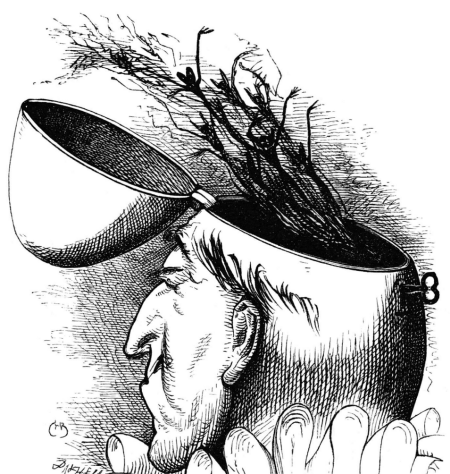
\includegraphics[scale=.35]{arcana/HollowHead}
\end{wrapfigure}


    Your brain disappears and your head has a hinge that opens like a box, but only you know this and only you can open it. For the rest of the Session,
    you are immune to the next \DICE Secrets of the Mind targeting you,  and you can fit up to \SUMDICE Burden inside of your head in \mylink{Hammerspace}{meta-hammerspace} (pulling one of these items out takes 1 Action).  When you resist the final Secret, the enchantment immediately ends. If the Secret ends while items are stored in your head, they will mix with your brain-matter. Usually this is fatal, though some Philosophers pack their head with \mylink{Narcotics}{gear-narcotics} and have a buddy speak a \mylink{Charm}{secrets-charm} Secret to them. While your head is hollow, another Philosopher could read any of the Secrets inscribed inside, just like your head was a Grimoire.

\newpage

\WIZARDRY[
  Name=Ice Bridge Step,
  Link=secrets-ice-bridge-step,
  Alignment=Elements,
  Save=N,
  Duration=Session,
  Counter=\mylink{Greaseball}{secrets-greaseball} ,
  Keywords=None,
  Target=Self
]

You and up to \DICE-1 allies can run over liquids as if they were land.  Ice forms beneath your feet with each step. If you slow down (to walk, fight,
etc), you'll sink. Very wavy seas may require you to \RSTRY{\DEX}.  Very hot liquids (like lava) may require you to \RSTRY{\INT}.  The ability is dispelled if you are struck by a Secret: Greaseball and you fail a Wizard Fight!.

\WIZARDRY[
  Name=Icebolt,
  Link=secrets-icebolt,
  Alignment=Elements,
  Save=Y (half),
  Duration=\DICE,
  Counter=None ,
  Keywords=None,
  Target=Close or Nearby point (straight line)
]

Throw a bolt of ice at a target Close or Nearby.  The bolt will travel in a straight line from your fingers.  Anything touched by the bolt takes
\SUMDICE damage, Save for half.  Additionally, everything that fails its Save is frozen to whatever surfaces they are touching.  Keys are frozen in
locks; swords are frozen to hands; boots are frozen to the ground (creatures are usually immobilized from the boots down unless they were
playing in a fountain or something).  The objects are stuck for the \Duration.

\WIZARDRY[
  Name=Illusion,
  Link=secrets-illusion,
  Alignment=Mind,
  Save=N,
  Duration=Varies,
  Counter=\mylink{Ego Weapon}{secrets-ego-weapon} ,
  Keywords=None,
  Target=Varies
]

You create an illusion of anything you desire. If anything touches the illusion, it will pass through it with no effect.  Think of the illusion as a perfectly accurate hologram that you are creating - the illusion can be
heard in addition to being seen, can perform the same action over and over again, and can deliver messages, but it can't interact in a meaningful way
or perform complex actions based on external forces. Each aspect of the illusion requires one or more Blood die to cast:

\callout{\footnotesize{

\mybullet {
  \item Having the illusion speak or make noise requires 1 \DICE for each word or sound (wailing, shouting, etc);
  \item Having the illusion appear to be a physical thing a (hole in the ground, a stone wall, orc guard, etc.) requires 1 \DICE for each square meter in size; 
  \item Having the illusion appear to move requires 1 \DICE for every meter;
  \item Having the illusion appear on a living creature (disguising them as a beggar or a lamp post) requires 1 \DICE, and they cannot be wearing or carrying any iron.
}}}

Note that there is some Arbiter's discretion here.  A guard pacing in front of a door might require 4 \DICE (a 2m tall "thing" pacing back and forth 2 meters), but more if you want them to appear more "natural" and not like a robot marching back and forth.  A disguise placed on someone to appear to be a beggar might cost 1 \DICE, but disguising yourself as the king will be significantly harder.

The Illusion will last for \DICE real-world hours.  Anyone touching the illusion will immediately know it to be fake, but this doesn't cause the illusion to disappear.  However, if the illusion is touched with an Ego Weapon, it will disappear if a Wizard Fight! is lost.


\WIZARDRY[
  Name=Invisibility,
  Link=secrets-invisibility,
  Alignment=Entropy,
  Save=N,
  Duration=\DICE,
  Counter=\mylink{Fool's Fire}{secrets-fools-fire} ,
  Keywords=None,
  Target=Self or Close Allies or Objects
]

Up to \DICE objects or creatures can be made \mylink{Invisible}{effect-invisible} (including yourself), and will remain that way as long as they don't move.  As soon as the creature or object moves (or is moved), the charm is broken.  Invisible creatures can see other invisible and hidden objects (including Knaves using Whispers).  

If this Secret is placed on something Invisible, it will force the object to become seen.  The duration of depends on the dice invested.  1 die: \SUMDICE Moments; 2 \DICE Minutes; 3 \DICE Hours; 4 \DICE Days; 5 \DICE Weeks; 6+ \DICE Forever.  The wisps from a Fool's Fire can dispel the Invisibility if a Wizard Fight! is lost.

  \myfpimage{arcana/Invisibility}


\WIZARDRY[
  Name=Kelsier's Swarm of Irritating Vermin,
  Link=secrets-kelsiers-swarm-of-irritating-vermin,
  Alignment=Force,
  Save=N,
  Duration=Combat or \SUMDICE real-world minutes,
  Counter=\mylink{Mighty Lungs}{secrets-mighty-lungs} ,
  Keywords=None,
  Target=Nearby; Far Away
]


You summon a cloud of tiny, magical, irritating vermin to an area Nearby or Far-Away.  The vermin deal \DICE damage per Moment to every living creature Close to them. If the target is an object, the vermin will do minor cosmetic damage, such as chewing holes in paper, gnawing wood, chipping paint, and scratching glass. Anything requiring Concentration is impossible within the Swarm, and any \mylink{Zoological Monsters}{monster-trait-zoological}  within the Swarm must make a Morale check or immediately flee somewhere Far-Away (this includes mounts and beasts of burden). The vermin won't move from the spot where they are summoned, and will remain until the Secret expires.  Mighty Lungs will dispel the swarm if a Wizard Fight! is lost.



\WIZARDRY[
  Name=Knife Trick,
  Link=secrets-knife-trick,
  Alignment=Force,
  Save=N,
  Duration=Session,
  Counter=\mylink{Grimm's Electric Fingers}{secrets-grimms-electric-fingers},
  Keywords=Splittable,
  Target=Close; Nearby; Far Away
]

Up to \DICE daggers orbit your head like a halo or crown (they cannot be iron).  These daggers must be in your possession, though "dagger-like" items are OK (icicles, shards of glass, etc.) at the Arbiter's discretion. At any time during the Session, you can mentally "throw" one or more of these daggers at things that are Close, Nearby, or Far-Away with unerring accuracy.  This could be used to sever a rope or pin something to a wall (or stick into someone's chest) - but no \mylink{Gambits}{combat-deeds-gambit}, that wouldn't be fair.  Each dagger does \SUMDICE+\DICE damage i.e. if you were to throw 1 dagger at someone, it would do d6+1, two daggers 2d6+2, etc.  \mylink{Grimm's Electric Fingers}{secrets-grimms-electric-fingers} will dispel the magic and cause the daggers to fall to the ground if a Wizard Fight! is lost.


\WIZARDRY[
  Name=Knock,
  Link=secrets-knock,
  Alignment=Entropy,
  Save=N,
  Duration=0,
  Counter=\mylink{Lock}{secrets-lock} ,
  Keywords=None,
  Target=Close or Nearby Objects
]


\DICE Close or Nearby object(s) is/are opened. Doors are flung wide, locks are broken, shackles are bent open, belts come undone.  Ideas or thoughts
can be unlocked from a mind if a \RBTRY{\INT}{\INT} contest is lost (target has a -\DICE penalty). Objects locked by Secret: Lock remain locked if a  Wizard Fight! is lost.


\WIZARDRY[
  Name=Levitating Disc,
  Link=secrets-levitating-disc,
  Alignment=Force,
  Save=N,
  Duration=Concentration,
  Counter=\mylink{Suspend Objects}{secrets-suspend-objects} ,
  Keywords=None,
  Target=Close or Nearby point in space
]


You draw a circle in the air of \DICE+\DICE diameter, in any orientation. The inside of the circle is made of Force, as solid as stone. You can cause the circle to raise, lower, or hover in place.  You can only move up and down (never side-to-side).  Up to \DICE people could stand under it and be completely covered, or on it and be levitated provided they don't weigh more than \DICE x200kg.  If you lower the circle on top of someone, they take \DICE damage
per Moment. The circle moves 10 meters a minute (about 3m per Moment).  You can change the disc's orientation at any time.  If the Levitating Disc is targeted with Suspend Objects, the disc will be dispelled if a Wizard Fight! is lost.


\WIZARDRY[
  Name=Lipby Chonk's Viscous Form,
  Link=secrets-lipby-chonks-viscous-form,
  Alignment=Biomancy,
  Save=N,
  Duration=Combat or \SUMDICE real-world minutes,
  Counter=None ,
  Keywords=None,
  Target=Self
]

Your flesh becomes gelatinous. You can squeeze through gaps as small as a keyhole with a great deal of effort. You take no damage from Crushing
attacks for the duration.  The Secret only affects your flesh, not anything you're wearing or carrying.


\WIZARDRY[
  Name=Lock,
  Link=secrets-lock,
  Alignment=Mind,
  Save=Y (negate),
  Duration=\DICE,
  Counter=None ,
  Keywords=None,
  Target=Close and Nearby Objects
]

Up to \DICE non-living thing slam shut and can't be opened for the \Duration. If the object is a door, chest, or something like it, it will slam shut forcefully and loudly. This Secret can work on things that aren't portals (a sword could be locked in its scabbard). You can also use this Secret to lock a specific memory or thought, making it immune to mind reading or scrying without a \RBTRY{\INT}{\INT}.  The Lock can be dispelled by the Secret: Knock if a Wizard Fight! is lost.


\WIZARDRY[
  Name=Meat Shield,
  Link=secrets-meat-shield,
  Alignment=Biomancy,
  Save=N,
  Duration=\DICE real-world hours,
  Counter=None ,
  Keywords=None,
  Target=Close and Nearby
]

You summon a giant slab of meat that fills an area \DICE meters cubed.  The meat weighs \DICE x100kg and lasts for \DICE real-world hours. \mylink{Zoological Monsters}{monster-trait-zoological} will attack the Meat Shield first. When the Meat Shield has been dealt \SUMDICE+\DICE damage or more to the Meat, consider it consumed/destroyed. During a \mylink{Bivouac}{combat-resting-bivouac}, up to \DICE Allies can eat the Meat Shield in lieu of rolling their Provisions, but the provenance of the meat is ... unknown.  If a Scything Disc of Nog is used on a Meat Shield, the shield will be dispelled if a Wizard Fight! is lost (otherwise, it will take damage as normal).

\WIZARDRY[
  Name=Mighty Lungs,
  Link=secrets-mighty-lungs,
  Alignment=Biomancy,
  Save=N,
  Duration=Until exhalation,
  Counter=None ,
  Keywords=Contested,
  Target=Self
]

Your next inhalation allows you inhale 10x the normal amount of air. Not only does this allow you to hold your breath for 10x as long, but if you
exhale forcefully it will release a blast of air strong enough to knock pigeons out of air and polish your teeth. A human-sized creature is knocked
\mylink{Prone}{effect-prone} and pushed Nearby unless they try a \RB \DEX or \VIG (their choice) with a -\DICE penalty vs your \INT.  This Secret will also blow open all closed but unlocked doors in a room, shatter all windows in a building, or knock the thatched roof off a peasant's shack.

\WIZARDRY[
  Name=Mirror Image,
  Link=secrets-mirror-image,
  Alignment=Entropy,
  Save=N,
  Duration=Session,
  Counter=None ,
  Keywords=None,
  Target=Self
]

You create \DICE illusory images of yourself, which move as you move and always stay Close to you. They are constantly stepping through each other,
making it impossible to determine which representation of you is "real". When an enemy attacks you, they'll always hit an image first.  An image vanishes as soon as it suffers
a solid impact (a blow from a mace, but also a slap). Area effects such as a dragon's breath will cause all images to instantly vanish (and you take the
damage, naturally). Finally, invoking \mylink{Mirror Image}{secrets-mirror-image} causes any other images that already exist to immediately vanish.


\WIZARDRY[
  Name=Morass,
  Link=secrets-morass,
  Alignment=Elements,
  Save=N,
  Duration=Concentration,
  Counter=\mylink{Bastogne's Glamping Charm}{secrets-bastognes-glamping-charm} ,
  Keywords=Contested,
  Target=Nearby or Far-Away Area
]

The ground \SUMDICE meters in radius and \DICE meters deep turns to black muck.  Monsters and objects in the mud sink 1 meter per Moment.  At the top of
the Moment, a creature can \RB: \VIG with a -\DICE penalty vs. your \INT to pull themselves out 1 meter (if they were only 1 meter deep to begin with, they escape).  If someone's head dips below the mud (2m for people, 1m for Pooka, 4m or more for giants), they immediately being drowning and must make a \DEATH roll at the top of every Moment they are submerged (they can still claw their way up 1m with a successful \RB try, as above).  If they don't have a \DEATH, they die in \HD Moments.

The Secret lasts for as long as you \mylink{Concentrate}{time-concentration}.  When you break your Concentration, everything that sunk in the mud is immediately vomited back to the surface. If the area covered by the Morass is targeted by Bastogne's Glamping Charm, the Morass will be dispelled (and the objects brought to the surface) if a Wizard Fight! is lost.


\WIZARDRY[
  Name=Negasonic Bomb,
  Link=secrets-negasonic-bomb,
  Alignment=Mind,
  Save=N,
  Duration=Concentration,
  Counter=\mylink{Cacophony}{secrets-cacophony} ,
  Keywords=None,
  Target=Nearby or Far Away Area
]

You roll a small orb of Mind to a point Close, Nearby or Far-Away; the orb rolls silently and is hard to see.  When the orb stops rolling it immediately and silently detonates.  Creatures Close to the designated point are \mylink{Deafened}{effect-deafened} until they move somewhere Nearby; likewise, no sound can be made (including speaking) while Close to the point of detonation. Arcana and skills that require vocalization are impossible within this area of silence, which lasts as long as you \mylink{Concentrate}{time-concentration}.  The bomb can be dispelled by Cacophony if a Wizard Fight! is lost.



\WIZARDRY[
  Name=Prismatic Ray,
  Link=secrets-prismatic-ray,
  Alignment=Entropy,
  Save=Y (half),
  Duration=0,
  Counter=None ,
  Keywords=Splittable,
  Target=Nearby or Far-Away
]

A brilliant white light emanates from your forehead to a point Nearby or Far-Away, where it splits into a prism of \DICE beams.  Each beam strikes a
random Monster Close to the prism (roll for each beam; a Monster can be hit by more than 1 beam).  Roll a d8 on the table below for each beam and apply its results.

\callout{\footnotesize{

\mynumlist {
  \item \mybold{Red} Target takes \DICE fire damage, Save for half. Highly flammable things catch fire.
  \item \mybold{Orange}  Target takes \DICE bashing damage, Save for half. 
  \item \mybold{Yellow} Target takes \DICE lightning damage, Save for half.  If you fail your Save, you drop what you're holding.
  \item \mybold{Green} Target takes \DICE acid damage, Save for half. Roll your Armor \UD if applicable.
  \item \mybold{Blue} Target takes \DICE ice damage, Save for half. If you fail your Save, you fall \mylink{Prone}{effect-prone}.
  \item \mybold{Indigo} Target takes \DICE stabbing damage, Save for half.
  \item \mybold{Violet} Target takes \DICE chopping damage, Save for half.
  \item \mybold{Roll} again.  Instead of \DICE damage, the effect deals \SUMDICE damage.. If you get this result again, the beam splits and the target takes an additional effect (roll again and apply the result).  Continue in this way until you don't roll an 8.
}}}


\WIZARDRY[
  Name=Pritchard's Gusty Belch,
  Link=secrets-pritchards-gusty-belch,
  Alignment=Biomancy,
  Save=N,
  Duration=0,
  Counter=None ,
  Keywords=None,
  Target=Close and Nearby Area
]

You can breathe out up to \DICE elements (fire, acid, water, wind, steam, etc) immediately in front of you for a Moment.  The elements don't interact with one another and act independently, so if you were to belch out fire and water, you would get the effects of both.  If the order matters (set something on fire and immediately douse it with water), you pick the order of effects.  Water breath is enough to extinguish fires smaller than a big bonfire, or wash off acid; wind breath could push a small sailboat or blow swarming insects out of an area; acid breath bleaches the color from objects and irritates the eyes; fire breath would cause paper and flammable objects (but not people, unless they were doused in oil) to catch fire, etc.


\WIZARDRY[
  Name=Protection from Element,
  Link=secrets-protection-from-element,
  Alignment=Elements,
  Save=N,
  Duration=Session,
  Counter=\mylink{Prismatic Ray}{secrets-prismatic-ray} ,
  Keywords=Splittable,
  Target=Self or Close Allies
]

Reduce all damage of a single chosen element (acid, cold, fire, lightning, etc) by -\DICE per die (minimum of 1).  The Secret protects its targets from the negative effects of the natural elements (desert heat, arctic chill) as well.  If you are struck by a Prismatic Ray of the same elemental type, the protection is dispelled if a Wizard Fight! is lost.

\myfpimage{arcana/Wizardry_1}



\WIZARDRY[
  Name=Rhea's Efficacious Plow,
  Link=secrets-rheas-efficacious-plow,
  Alignment=Force,
  Save=N,
  Duration=Moments,
  Counter=None ,
  Keywords=None,
  Target=See description
]

You send an invisible wedge of Force along the ground in a straight line up to a Distant point. The wedge can take up to \DICE left or right turns at your command. Any light debris in the path (snow, small stones, leaves, grass) is pushed to the side; fields can be tilled. Any pressure plates or tripwires are activated. You do not have to be able to see the entire path, but you do need to know the approximate route the wedge will take. The wedge can't move through solid objects, and it can't directly hurt anyone (though it will push them to the side). The path cleared is \DICE meters wide. If you cast this Secret with 3+ \DICE, the width becomes \SUMDICE meters wide.

\WIZARDRY[
  Name=Sandstorm,
  Link=secrets-sandstorm,
  Alignment=Elements,
  Save=N,
  Duration=Concentration,
  Counter=None ,
  Keywords=None,
  Target=Close
]

You cough up a swirling spiral of sand.  Small flying creatures (bug-sized) and missile weapons cannot enter or leave the sandstorm.  Up to \DICE-1 other
people can hide in the sandstorm with you.  The sand moves with you and lasts as long as you \mylink{Concentrate}{time-concentration}.



\WIZARDRY[
  Name=Sanguine Mail,
  Link=secrets-sanguine-mail,
  Alignment=Biomancy,
  Save=N,
  Duration=Session or until Exhausted,
  Counter=\mylink{Enervate}{secrets-enervate} ,
  Keywords=None,
  Target=Self
]


You become encased in elaborate plate mail that seems to be made from constantly congealing blood.  You definitely stand out in a crowd. Your \MD drops to d8.  The \UD for the Armor depends on the number of \DICE invested: 1 d4; 2 d8; 3+ d12. You can only have one Sanguine Mail active at a time. If you are struck with an Enervate spell, the Sanguine Mail is dispelled if a Wizard Fight! is lost.


\WIZARDRY[
  Name=Scuttle,
  Link=secrets-scuttle,
  Alignment=Biomancy,
  Save=N,
  Duration=Combat or \SUMDICE real-world minutes,
  Counter=\mylink{Greaseball}{secrets-greaseball} ,
  Keywords=None,
  Target=Self
]


Your clothes and hair animate to carry you around. You can move at full speed in any orientation, and you can freely rotate as you move. For
instance, you could run while standing on your head, holding a torch, and turning counterclockwise. You can lie on your side and, while flipping end
over end, move backwards. This effect does not allow you to climb up walls, but ladders and ropes are no problem (you could suspend yourself from a rope
and cast spells, for example).  If you are struck with a Greaseball, or attempt to climb something affected by Greaseball, the Scuttle is dispelled if a Wizard Fight! is lost.




\WIZARDRY[
  Name=Scything Disc of Nog,
  Link=secrets-scything-disc-of-nog,
  Alignment=Force,
  Save=Y (half),
  Duration=0,
  Counter=None ,
  Keywords=None,
  Target=Nearby or Far Away Area
]

You hurl a whirling disc of Force and light from your fingertip. The disc screeches like a sawblade. It deals \SUMDICE damage to its target, Save for
half. If it deals more than 6 damage, it bounces towards a random creature (friend, foe, or even yourself) Close or Nearby, dealing \SUMDICE-2
damage, Save for half. If it deals more than 6 damage, it bounces towards another random creature Close or Nearby, dealing \SUMDICE-4 damage, Save for
half. This continues, losing 2 damage with each bounce, until there are no valid targets or the Secret deals 6 or less damage to a creature.


\WIZARDRY[
  Name=Sleep,
  Link=secrets-sleep,
  Alignment=Mind,
  Save=Y (negate),
  Duration=\DICE,
  Counter=\mylink{Cacophony}{secrets-cacophony} ,
  Keywords=None,
  Target=Close or Nearby Area
]

You summon a cloud of somnolent dust to a point Close or Nearby. \SUMDICE creatures Close to the cloud, who have no more than \DICE \mylink{Hit Dice}{monster-hit-dice}, must
immediately Save or fall into a magical slumber.   They can't be awakened by anything less than a vigorous slap (counts as 1 Action).  You don't have
control over who falls asleep, it's entirely random - but will be as many creatures as possible (up to \SUMDICE), which means lower \HD creatures will go to sleep first.  You are immune to your own Secret: Sleep (so you could cast it Close to yourself).  Creatures who fall asleep immediately fall \mylink{Prone}{effect-prone} and drop any items they're holding.  Attack tries against them will hit automatically and do maximum damage, and can only be blocked by Armor.  This will wake the creature up, of course.  If an orb of Cacophony is detonated Nearby, the creatures will awaken if a Wizard Fight! is lost.  Otherwise, creatures who fall asleep will remain asleep for the \Duration.  


\WIZARDRY[
  Name=Summon Candles,
  Link=secrets-summon-candles,
  Alignment=Force,
  Save=N,
  Duration=Session or until used,
  Counter=\mylink{Fogbank}{secrets-fogbank} ,
  Keywords=None,
  Target=Close
]

\SUMDICE dribbling candles appear on objects you touch. You can walk around placing candles as required for Minutes. The candles are lit and burn for
the entire Session (though see below). They can be detached, but will fade from existence within Minutes unless reattached.  

For every 6 candles that are Nearby to you, you may do one of the following:

\callout{\footnotesize{

\mybullet {
    \item Gain a +4 on a Wizard Fight! try;
    \item Cause a physical attack that would hit you to miss instead; 
    \item \mylink{Nudge}{dice-nudge} one of your rolled Blood Dice to a natural 6;
    \item Reduce a Ruin to a Calamity; a Calamity to a Mishap; or take no effect from a Mishap
}}}

When you use any of these powers, 6 candles immediately disappear. You must have at least 6 candles Nearby to use a power (no "rounding up"). The candles disappear at the end of the Session if they're not used. Candles encased in a Fogbank are snuffed out and dispelled if a Wizard Fight! is lost.


\WIZARDRY[
  Name=Suspend Objects,
  Link=secrets-suspend-objects,
  Alignment=Force,
  Save=Y (negate),
  Duration=Concentration,
  Counter=\mylink{Levitating Disc}{secrets-levitating-disc} ,
  Keywords=None,
  Target=Any Distance
]


You can hold up to \DICE objects in the air, weighing no more than \DICE x200kg.  You can allow these objects to descend at 3m per Moment at your
discretion. Creatures who are brought to ground in this way take no damage from \mylink{Falling}{movement-falling}. Unwilling creatures (flying Monsters, for example) get a Save to negate if you attempt to force them to the ground.  If a Levitating Disc is summoned in the midst of the held creatures, the Secret: Suspend Objects will be dispelled (and the objects will fall) if a Wizard Fight! is lost.


\WIZARDRY[
  Name=Tempestuous Chariot,
  Link=secrets-tempestuous-chariot,
  Alignment=Elements,
  Save=N,
  Duration=One trip,
  Counter=None ,
  Keywords=None,
  Target=Close
]

A tumult of air elementals lifts you and \DICE-1 others and takes you in any direction you desire, up to \SUMDICE km away.   One catch - the elementals can only travel in a straight line, and you have to choose beforehand the way to go ("up", "east", "that way", etc).  While you are in the tempest you are buffeted horribly and can neither talk nor act.  The winds refuse to travel without you, and will immediately dispel if you lose contact.


\WIZARDRY[
  Name=Vertigo,
  Link=secrets-vertigo,
  Alignment=Mind,
  Save=Y (negate),
  Duration=\DICE,
  Counter=\mylink{Suspend Objects}{secrets-suspend-objects} ,
  Keywords=None,
  Target= Any Distance
]

You can cause up to \DICE Close, Nearby, Far-Away, or Distant creatures to suffer severe vertigo unless they Save.  Creatures that are climbing or
flying immediately fall; creatures who are Close to the edge of something (a cliff, a wall, the guardrails of a ship, etc) need to \RSTRY{\FOC} or fall.
Creatures already on the ground will fall \mylink{Prone}{effect-prone} for the \Duration. If the creatures are struck with a Suspend Objects spell, the Vertigo is dispelled if a Wizard Fight! is lost.

\newpage

\WIZARDRY[
  Name=Web,
  Link=secrets-web,
  Alignment=Entropy,
  Save=Y (negate),
  Duration=\DICE,
  Counter=None ,
  Keywords=None,
  Target=Nearby or Far Away Area
]

You can anchor a giant web between three or more solid points up to \DICE meters in radius (for example: the 4 points of a door, two trees and the ground, across a hallway, etc).  Objects that touch the web immediately become stuck; arrows and spears can't be fired through it.  Creatures that enter the web (or are caught in it when cast) must Save or become ensnared for \Duration (each creature must make its \Duration try separately). Attack tries against them hit automatically and can only be blocked by Armor.  The web is extremely flammable and will be consumed in \DICE Moments.

\myfpimage{arcana/Spider}

\WIZARDRY[
  Name=Whirling Blades,
  Link=secrets-whirling-blades,
  Alignment=Entropy,
  Save=N,
  Duration=Concentration,
  Counter=\mylink{Suspend Objects}{secrets-suspend-objects} ,
  Keywords=None,
  Target=Self
]

You summon a number of invisible blades of Force that spin around your waist, with you in the center.  Every creature Close to you takes \DICE+\DICE
damage for each Moment the Secret is maintained.  The blades will cut or damage fragile objects.  If the creature or object sits above or below your waist, they take no effect.  If the blades are struck by a Secret: Suspend Objects, they will be dispelled if a Wizard Fight! is lost.

\begin{multicols}{2}
